% !TEX root = ../notes.tex

Here we go.

\subsection{Finishing Completeness}

Today we are continuing the proof of \autoref{thm:langcomplete}.
\langcomplete*
\begin{proof}
	Here is the idea: suppose that $f:\{0,1\}^n\to\{0,1\}$ is a truth function. Because it has finitely many inputs, the pre-image of $\{1\}$ is finite, so we enumerate them by
	\[r_1,\ldots,r_m,\]
	where the ``row'' $r_k$ is the input $(b_{k1},\ldots,b_{km})$. With this, we define
	\[\varphi_{r_k}:=\pm p_1\land\cdots\land p_m,\]
	where we take $+p_\bullet=p_\bullet$ if and only if $b_{k\bullet}=1$ and $-p_\bullet=\lnot p_\bullet$ otherwise.
	\begin{definition}[Literal]
		A formula of the form $p,\lnot p\in\mathcal L(P)$ is called a \textit{literal}.
	\end{definition}
	The point is that $\varphi_{r_k}$ is true if and only if the input is equal to $(b_1,\ldots,b_m)$. In particular, when we take
	\[\varphi:=\varphi_{r_1}\lor\cdots\lor\varphi_{r_m},\]
	we see that $\varphi$ is true if and only if one of the $\varphi_{r_\bullet}$ is true if and only if one of the inputs is equal to $r_\bullet$. So $\varphi$ defines the truth function $f$.
\end{proof}

\subsection{Normal Forms}
We have the following corollary of \autoref{thm:langcomplete}.
\begin{corollary}[Disjunctive normal form] \label{cor:dnf}
	Fix $P$ a finite set. Every truth function $P\to\{0,1\}$ can be represented by using $\lnot,\lor,\land$ as a disjunction of conjuction of literals.
\end{corollary}
Recall that disjunction means $\lor$ (having one but not the other is legal), and conjunction means $\land$ (we must have both).
\begin{proof}
	This is exactly what \autoref{thm:langcomplete} does: it produces conjucntions of literals and then disjunts them together.
\end{proof}
\begin{definition}[Disjunctive normal form]
	A formula $\varphi$ which is a disjunction of a conjunction of literals is said to be in \textit{disjunctive normal form}.
\end{definition}
\begin{example}
	Disjunctive normal form is not unique. For example,
	\[(p\land q\land r)\lor(p\land q\land\lnot r)\lor(\lnot p\land q\land r)\lor(\lnot p\land\lnot q\land r)\]
	is equivalent to
	\[(\lnot p\land q\land r)\lor(\lnot p\land\lnot q\land r),\]
	both of which are in disjunctive normal form.
\end{example}
There is also a dual notion to disjunctive normal form.
\begin{definition}[Conjunctive normal form]
	A formula $\varphi$ which is a conjuction of a disjunction of literals is said to be in \textit{disjunctive normal form}.
\end{definition}
To put a formula into conjunctive normal form, we can put $\lnot\varphi$ into disjunctive normal form as
\[\lnot\varphi\equiv\bigvee_{k=1}^m(\ell_{k,1}\land\cdots\land\ell_{k,n}).\]
In other words, we look for all the $0$s in the truth table. Then we negate to take
\[\varphi\equiv\bigwedge_{k=1}^m(\ell_{k,1}'\lor\cdots\lor\ell_{k,n}'),\]
which is our conjunctive normal form, where $\ell_{k,\bullet}'$ is the negated literal.
\begin{example}
	Consider the truth table as follows.
	\[\begin{array}{c|c|c||c}
		p & q & r & f \\
		\hline
		1 & 1 & 1 & 1 \\
		1 & 1 & 0 & 1 \\
		1 & 0 & 1 & 0 \\
		1 & 0 & 0 & 0 \\
		0 & 1 & 1 & 1 \\
		0 & 1 & 0 & 0 \\
		0 & 0 & 1 & 1 \\
		0 & 0 & 0 & 0
	\end{array}\]
	Our zeroes are at
	\[\lnot\varphi\equiv(p\land\lnot q\land r)\lor(p\land\lnot q\land\lnot r)\lor(\lnot p\land q\land\lnot r)\lor(\lnot p\land\lnot q\land\lnot r).\]
	Negating and applying de Morgan's laws, our formula is
	\[\varphi\equiv(\lnot p\lor q\lor\lnot r)\land(\lnot p\lor q\lor r)\land( p\lor\lnot q\lor r)\land( p\lor q\lor r).\]
\end{example}

We close by noting our proof of \autoref{thm:langcomplete} finishes the exactness in the proof of \autoref{cor:countequivclasses}. To be more explicit, we showed that there are at most $2^{2^n}$ different equivalent formulae because this is the number of truth functions, but \autoref{thm:langcomplete} showed that all truth functions are possible. So there are indeed $2^{2^n}$ total different equivalence classes of formulae.

\subsection{Our Gates}
Let's start talking about some digital circuits. We start with some gates.
\begin{definition}[NOT gate]
	The \textit{NOT gate} (or inverter) is a gate which takes low voltage to high voltage and vice versa.
	\begin{center}
		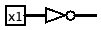
\includegraphics[scale=0.5]{not.png}
	\end{center}
\end{definition}
\begin{definition}[AND gate]
	The \textit{AND gate} is a gate which takes high voltage if and only if both of its inputs are high voltage.
	\begin{center}
		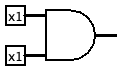
\includegraphics[scale=0.5]{and.png}
	\end{center}
\end{definition}
\begin{definition}[OR gate]
	The \textit{OR gate} is a gate which takes high voltage if and only if at least one of its inputs are high voltage.
	\begin{center}
		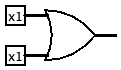
\includegraphics[scale=0.5]{or.png}
	\end{center}
\end{definition}
\begin{definition}[NAND gate]
	The \textit{NAND gate} is a gate which takes high voltage if and only if at least one of its inputs are low voltage.
	\begin{center}
		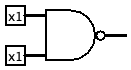
\includegraphics[scale=0.5]{nand.png}
	\end{center}
\end{definition}
\begin{definition}[NOR gate]
	The \textit{NOR gate} is a gate which behaves like negative of the OR gate.
	\begin{center}
		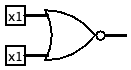
\includegraphics[scale=0.5]{nor.png}
	\end{center}
\end{definition}
\begin{definition}[XOR gate]
	The \textit{XOR gate} is a gate which has high voltage if and only if exactly one of the inputs is high-voltage.
	\begin{center}
		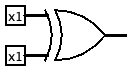
\includegraphics[scale=0.5]{xor.png}
	\end{center}
\end{definition}
\begin{definition}[XNOR gate]
	The \textit{XNOR gate} is a gate which has high voltage if and only if its inputs have the same voltage.
	\begin{center}
		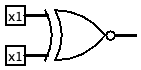
\includegraphics[scale=0.5]{xnor.png}
	\end{center}
\end{definition}


\subsection{Building Circuits}
We can connect these circuits together in fun ways.
\begin{center}
	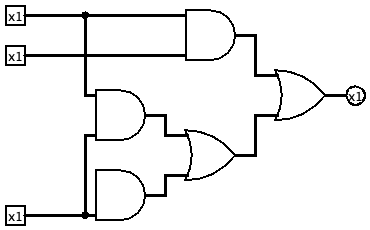
\includegraphics[scale=0.5]{majority.png}
\end{center}
Reading off of this circuit corresponds gives the formula
\[(p\land q)\lor((p\land r)\lor(q\land r)).\]

Let's see an example problem.
\begin{exe}
	We build a circuit with two switches such that either light switch turns the lightbulb on or off.
\end{exe}
\begin{proof}
	It is not too implausible to think that we can do this with a formula because we are essentially asking for the number of ``on'' light-switches to be odd to give the light-bulb on. Here is a circuit which works.
	\begin{center}
		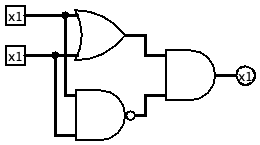
\includegraphics[scale=0.5]{lights.png}
	\end{center}
	It corresponds to the formula $(p\lor q)\land\lnot(p\land q)$. This is essentially an XOR gate.
\end{proof}
It is possible for circuits to be inefficient. For example, consider the following circuit.
\begin{center}
	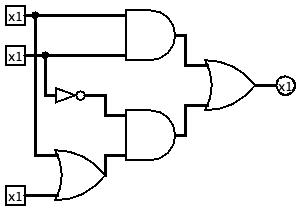
\includegraphics[scale=0.5]{complex.png}
\end{center}
This can be simplified down. Indeed, this corresponds to the formula
\[(p\land q)\lor(\lnot q\land(p\lor r)).\]
We can argue that this is equivalent to
\[p\lor(\lnot q\land r)\]
by doing some simplification. Thus, we can build the following simpler circuit.
\begin{center}
	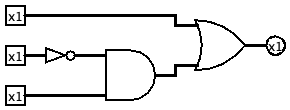
\includegraphics[scale=0.5]{simpler.png}
\end{center}
So this is an application of simplifying formulae.
\begin{remark}
	We remark that any formula can be written using $\uparrow$, which corresponds to the fact that all circuit functions could be written in only NAND gates.
\end{remark}
\begin{remark}
	One can build the same theory of equivalence and so on of circuits by porting over the theory from formulae/truth functions to circuits.
\end{remark}